\subsection{Temporal stability}
The following section will give a brief insight in to the effects of choosing different $\theta$ values in the $\theta-$scheme. The benchmark test FSI-2 has been used to since it is known to blow up with certain values of $\theta$ and $\Delta t$. Only the effects of Drag as been studied as the three other quantities shows the same behavior.   


\begin{figure}[H]  \label{fig:FSI2drag_plots} 
  \caption {Drag for FSI2 with $\Delta t = 0.01$ with different values for $\theta$}
  \begin{minipage}[b]{0.5\linewidth}
    \centering
    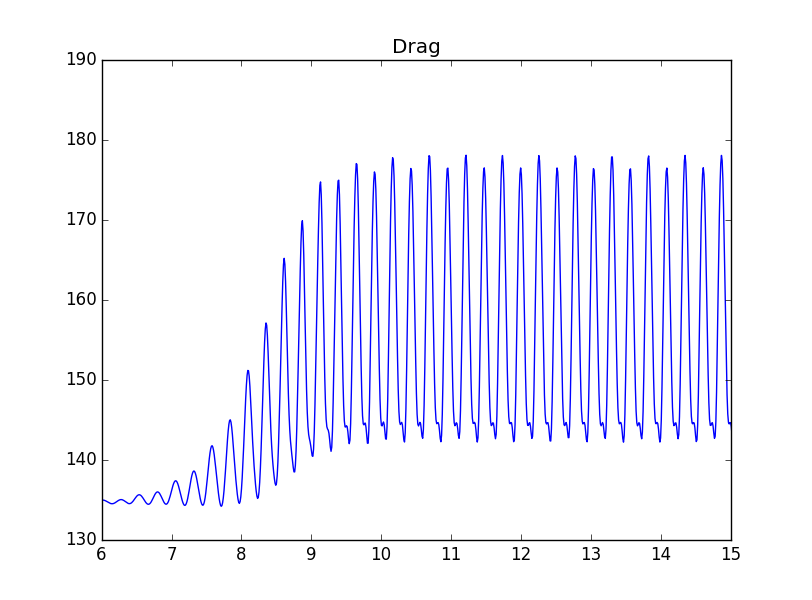
\includegraphics[scale=0.35]{./Verification_Validation/Temporal_stability/FSI2_001_051_big.png} 
    \caption{$\theta = 0.51 $} 
    \vspace{4ex}
  \end{minipage}%%
  \begin{minipage}[b]{0.5\linewidth}
    \centering
    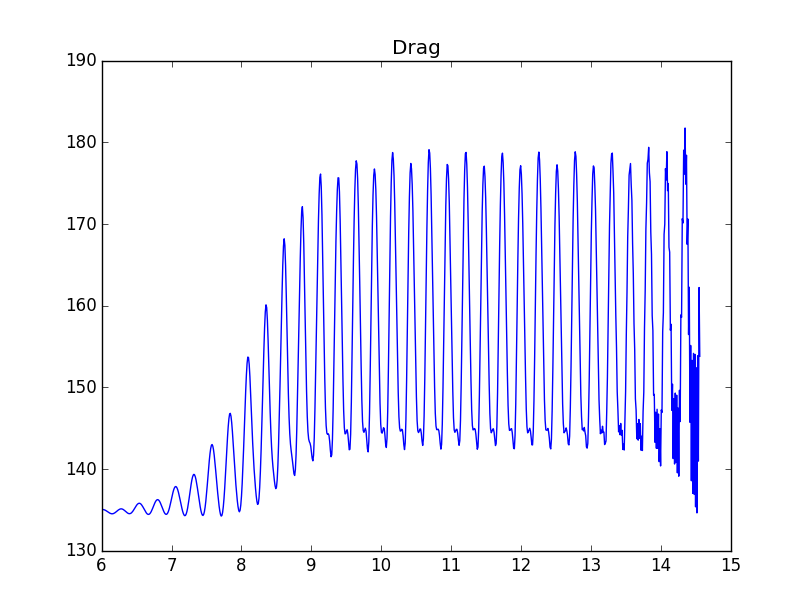
\includegraphics[scale=0.35]{./Verification_Validation/Temporal_stability/FSI2_001_050_big.png} 
    \caption{$\theta = 0.50 $} 
    \vspace{4ex}
  \end{minipage} 
  \begin{minipage}[b]{0.5\linewidth}
    \centering
    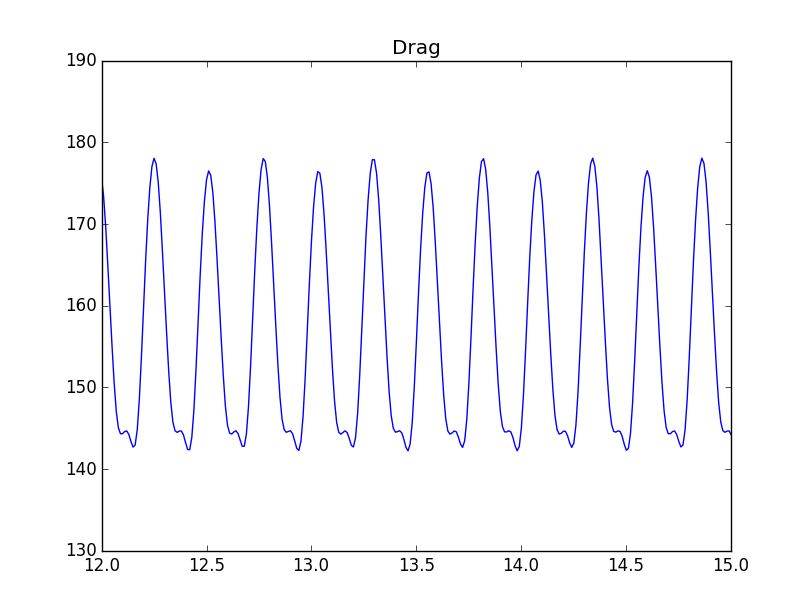
\includegraphics[scale=0.35]{./Verification_Validation/Temporal_stability/FSI2_001_051_small.png} 
    \caption{$\theta = 0.51 $} 
    \vspace{4ex}
  \end{minipage}%% 
  \begin{minipage}[b]{0.5\linewidth}
    \centering
    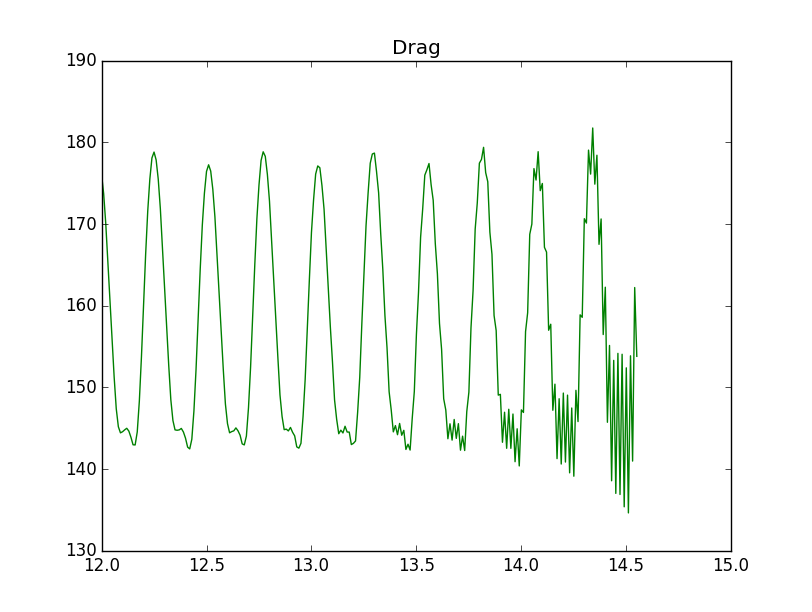
\includegraphics[scale=0.35]{./Verification_Validation/Temporal_stability/FSI2_001_050_small.png} 
    \caption{$\theta = 0.50 $} 
    \vspace{4ex}
  \end{minipage} 
\end{figure}


\ref{fig:FSI2drag_plots} show the plots of Drag with $\Delta t = 0.01$. It shows the instability when choosing $\theta = 0.5$. The Crank-Nicholson scheme is stable until about 13 seconds where we see that it blows up and the solver diverges. While the shifted Crank-Nicholson, $\theta = 0.5 + \Delta t$, is stable throughout the computing time.\newline

It has been reported in \cite{Wick2011} that the Crank-Nicholson, $\theta = 0.5$, scheme is stable throughout the computing time by setting $\Delta t = 0.001$.

Put in plot of $\theta = 0.5$ and $\Delta t = 0.001$ to see if its stable longer? +++++++
